\documentclass[a4paper, 11pt, fleqn]{article}
\usepackage{custom}
\usepackage{titlepage}
\usepackage{import}
\usepackage{tikz}
\usepackage[bottom]{footmisc}
\usepackage{tabu}
\usepackage{wrapfig}
\usepackage{apacite}
\hypersetup{%
	pdfborder = {0 0 0}
}
\usepackage[default]{sourcesanspro}
\usepackage[T1]{fontenc}
\normalfont
%============STYLE PROPERTIES============
\setlength{\parindent}{0pt}
\graphicspath{{pdf/}{images/}}
%============PAGE PROPERTIES=============
\newcommand{\revisiondate}{\today}
\newcommand{\documenttitle}{Sustainability } % used for title in title and subtitle pages
\newcommand{\authors}{Group 05} %used for title page only
\newcommand{\subauthors}{Lukas Tanner\\Sandro Holderegger\\ Daniel Hediger\\ Heinz No\"{e}l} % used for titlepage only
\newcommand{\subtitle}{Final Report} % used for title and subtitle pages
\newcommand{\documentdesc}{\textbf{THE LIFECYCLE OF WINE}}
\newcommand{\titleimg}{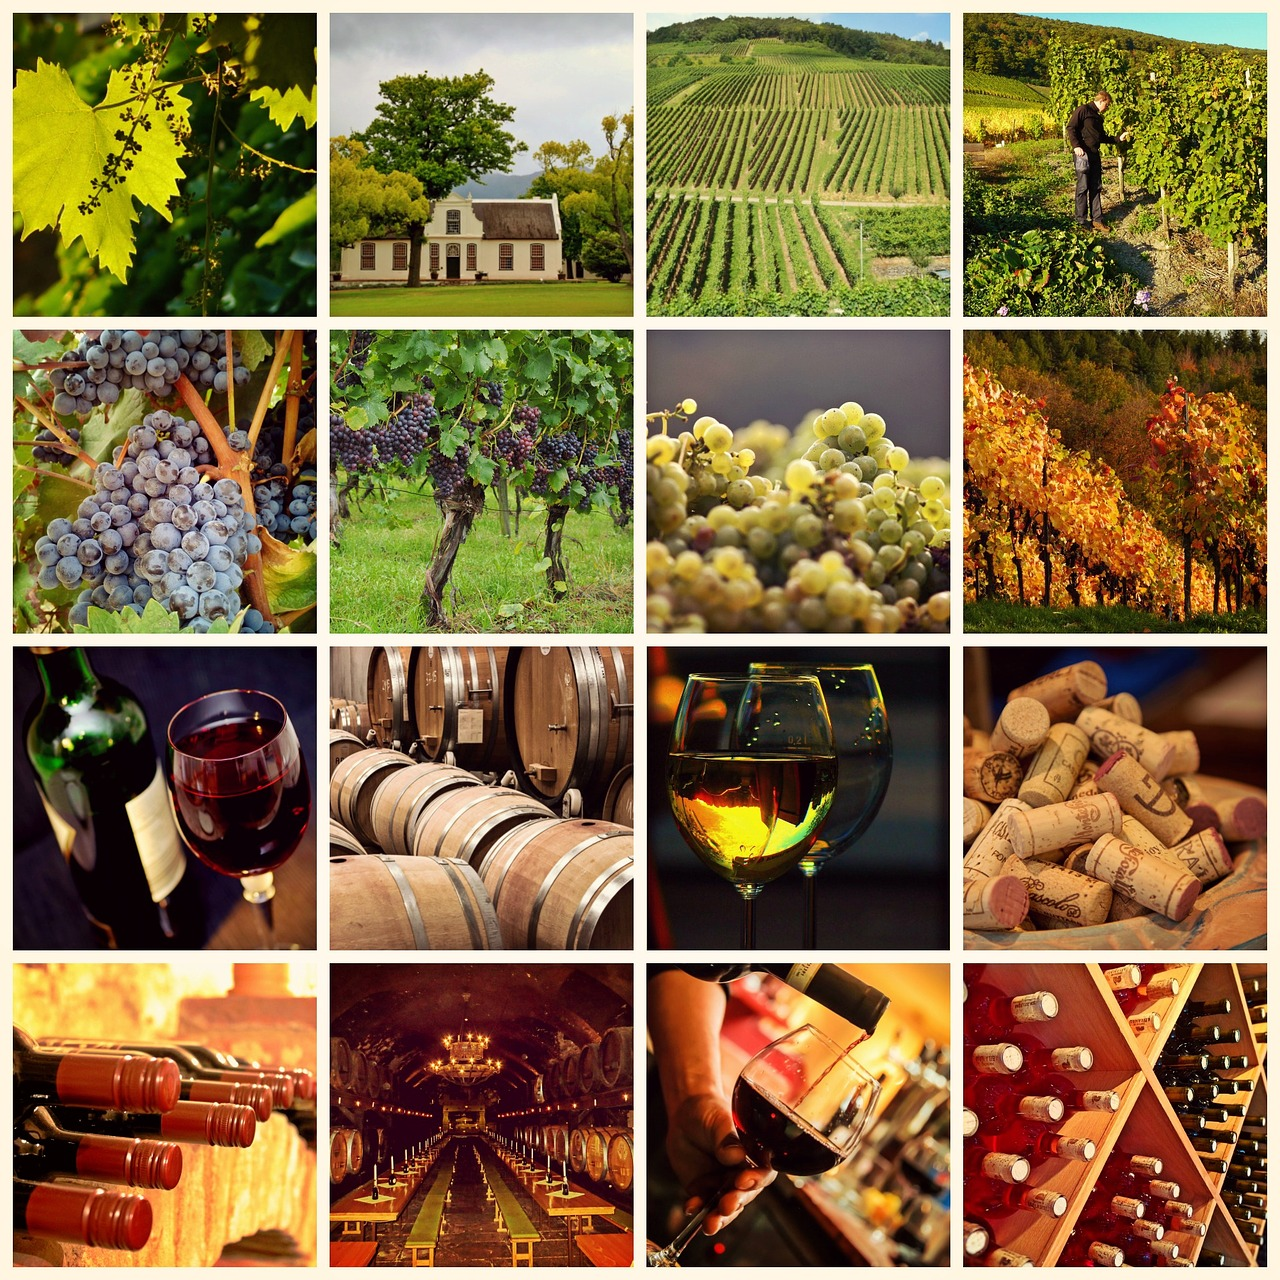
\includegraphics[width=.5\textwidth]{titlepage.jpg}}
\newcommand{\dozent}{Dr. Ulrike Sturm}
\newcommand{\ort}{Hochschule Luzern Technik \& Architektur, Horw}
 \renewcommand{\baselinestretch}{1.50}\normalsize
 \bfseries
    
\begin{document}
	\begin{titlepage}
	\titleGM
	\thispagestyle{empty}
	\end{titlepage}
		\tableofcontents	
\clearpage
\section{Einleitung}

Die Schweizer legen einen grossen Wert auf naturnahes und nachhaltiges Anbauen von
landwirtschaftlichen Gütern. Es gibt kurze Transportwege, genügend Wasser, die Recycling-Quote ist
hoch und die Konsumenten sind sich ihrer Verantwortung bewusst. Die Arbeiter geniessen einen
Mindestlohn, sind sozialversichert und können auf eine gute Rente hoffen.

In Kalifornien hingegen wohnen Amerikaner. Die sind verschwenderisch und kümmern sich nicht um ihre
Umwelt. Sie werfen alles weg und woher die Rohstoffen kommen, ist ihnen egal. Die Arbeit wird von
illegalen Mexikanern verrichtet, die weder ein geregeltes Einkommen haben noch sich gewerkschaftlich
organisieren dürfen.

Soweit die Vorurteile. Nach dieser oberflächlichen Betrachtung ist es eigentlich klar, welcher Wein
aus ökologischen und sozialen Gründen gekauft werden sollte. Doch hält diese Schlussfolgerung auch
einer Life Cycle Analyse stand? Diese Frage soll dieser Report beantworten.

\newpage
	\section{Life Cycle Analyse}
	In diesem Kapitel wird Lebenszyklus einer Weinflasche untersucht Von dem Anbau bis zum Genuss an einem romantischen Dinner, wird jeder Vorgang einzeln unter die Lupe genommen und sich Gedanken gemacht wie Nachhaltig dieses Luxusgut eigentlich ist. Die Arbeitsschritte wurden Analysiert und die wichtigsten Aspekte in den nachfolgenden Kapiteln untersucht. Es wird versucht aufzuzeigen was für Emission dabei überhaupt entstehen.
\subsection{Transport}
In diesem Abschnitt wird betrachtet welchen Weg eine Flasche von Kalifornien zurücklegt bis bei einem Einzelhändler in Konstanz im Regal entsteht. Hauptaspekt in dieser Betrachtung ist der entstandene Co2 Ausstoss pro Flasche Wein. Grundlage hier dient die \cite{_kohlendioxid-bilanz}. 
\begin{description}
	\item[1 Station]\hfill \\
	Flaschenabfüllung beim Weinbaubetrieb in Acampo, San Joaquin County, 			Kalifornien und sechs Kilometer Transport per LKW (Beladung mit 4.704 			Flaschen) zum Ravenswood-Distribution-Center in Lodi, San Joaquin 				County, Kalifornien
	\item[2 Station]\hfill \\
	Beladung eines 20-PANAMAX-Containers mit insgesamt 12.768 Flaschen 			und 140 Kilometer LKW-Transport des Containers zum Port of Oakland, 			Kalifornien.
	\item[3 Station]\hfill \\
		17.283 Kilometer Seetransport des Containers von Oakland über Panama 			zum Europoort Rotterdam, Niederlande;
	\item[4 Station]\hfill \\
		Umladung des Containers auf ein Rheinschiff und 487 Kilometer Transport 			nach Mainz sowie	
	\item[5 Station]\hfill \\ 
	152 Kilometer LKW-Transport des 20-Fuß-Containers von Mainz bis zum 			Weinhändler nahe Koblenz
\end{description}

Ergebnis einer Studie der Justus-Liebig-Universität Gießen (JLU) in Kooperation mit der San Francisco State University: Der globale Transport einer Flasche kalifornischer Wein über 18.000 Kilometer vom Abfüller in Kalifornien bis zum Einzelhandel gerade einmal 200 Gramm Kohlendioxid zuzurechnen. 200 Gramm Kohlendioxid werden beispielsweise frei, wenn ein privater PKW eine Strecke von nur 1,4 Kilometer zurücklegt.   \cite{_kohlendioxid-bilanz}. 


CO2 Ausstoss bei der Produktion
Bei der Produktion von Wein fallen durch verschiedene Arbeitsprozesse CO2 Emissionen an. Solche Arbeitsprozesse sind z.B Beschaffung und Verteilung von Dünger mit einem Traktor, Transport der Arbeitskräfte an den Einsatz Ort, Abtransport der Ernte. All dies sind Faktoren die einen unter anderem einen Ausstoss von Kohlendioxid zur Folge haben. In der Schweiz liegt dieser Wert pro ein Kilogramm produzierten Weintrauben zwischen 0.45 kg CO2-eq/Flasche und 0.6 kg CO2-eq/Flasche (ADEME, 2015). Die Variation entsteht durch die verschiedenen Traubensorten welche angebaut werden. In Kalifornien liegt dieser Wert bei 0.3 kg CO2-eq/Flasche bei der Lodi Sorte und bei 0.675 kg CO2-eq/Flasche bei der Napa Sorte.
Anhand dieser Zahlen kann man sagen das der Wein welcher in Kalifornien produziert wird ein bisschen weniger umweltbelastend ist als solcher in der Schweiz. Als Konsument muss sollte man aber beachten das der Wein aus Kalifornien durch seine lange Reise noch um die 0.2 kg CO2-eq/Flasche dazukommen. Dieser Wert ist entgegen der Erwartung eher klein, dies liegt daran das die Weinflaschen hauptsächlich im grossen Verbund auf einem Containerschiff den Grossteil der Strecke zurücklegen.Dazu kommt das nur ein nur ein kleiner Prozentsatz(unter 2\%) des Schweizer Weines exportiert wird und der grossteil direkt in der Schweiz verwertet wird. Die dadurch verursachten Emissionen sind dadurch minimal. 
\clearpage
	\subsection{Löhne}
Da Nachhaltigkeit sich nicht nur auf die Umwelt bezieht, sondern auch auf die Bereiche Sozial und Wirtschaft bezieht, untersuchen wir in diesem Abschnitt der Arbeit die Löhne und die Arbeitsbedingungen der Arbeitnehmer der Weinanbaubranche jeweils in der Schweiz und Kalifornien.

\subsubsection{Schweiz}
In der Schweiz sind die Lebensgrundkosten sehr hoch, und dafür ist es wichtig dass die Arbeiter angemessen bezahlt werden um zu gewährleisten dass ein gewissen Lebensstandard einzuhalten. Unter dem Motto "Ein glücklicher Mitarbeiter ist ein produktiver Mitarbeiter " werden in der Schweiz gemäss
\cite{_branchenverband} auch anständige Löhne für die hiesigen Mitarbeiter bezahlt. Mit einem Einstiegslohn von rund 4700 Schweizer Franken pro Monat, werden Winzer auch für die körperlich anstrengende Arbeit gerecht entlohnt. Durch das schweizerische Dreisäulensystem dient als angemessene Sicherung des Existenzbedarf und gilt als Sicherheit für die Arbeiter. Im ganzen gesehen ist der Beruf des Winzers in der Schweiz als sicher zu betrachtet. In der Schweiz wird der Wein oft in KMUs produziert oder in Familienunternehmen. In der Region Schweiz wird Wein seit den Römern produziert. 1

\subsubsection{Kalifornien}

Der durchschnittliche Verdienst in den Vereinigten Staaten von Amerika beträgt rund um die 3080 US Dollar pro Monat. \cite{_assistant} Dieser Betrag schwankt ein wenig von Staat zu Staat, aber dient hier nur als Vergleich. Bezüglich des Verdienstes spielt es in der kalifornischen Weinproduktion eine essenzielle Rolle welchen Beruf ausgeübt wird. So verdient ein sogenannter «Winemaker», was der Chef einer Kellerei ist, um die 9000 US
Dollar und ein Assistent um die 5 730 US Dollar pro Monat. Diese Werte liegen beide ziemlich weit über den weiter oben genannten Nationalen Durchschnitt. Zu beachten gilt hier dass nur wenige Personen diese Berufung pro Kellerei ausüben. Der Grossteil der Arbeit
wird von sogenannten «grape picker» verrichtet. Diese Pflücken die Weintrauben auf dem Feld. Ein solcher Feldarbeiter verdient im Durchschnitt circa 10 US Dollar pro Stunde,
\cite{_farm} hochgerechnet auf ein pro Monat macht das 1500 US Dollar, dies ist um einiges weniger als der D
urchschnitt. Die harte Feldarbeit wird zu einem grossen Teil von mexikanischen Immigranten verrichtet, ähnlich in Spanien bei welchen die Feldarbeit von polnischen Immigranten verrichtet wird.
\begin{figure}[H]
	\centering
	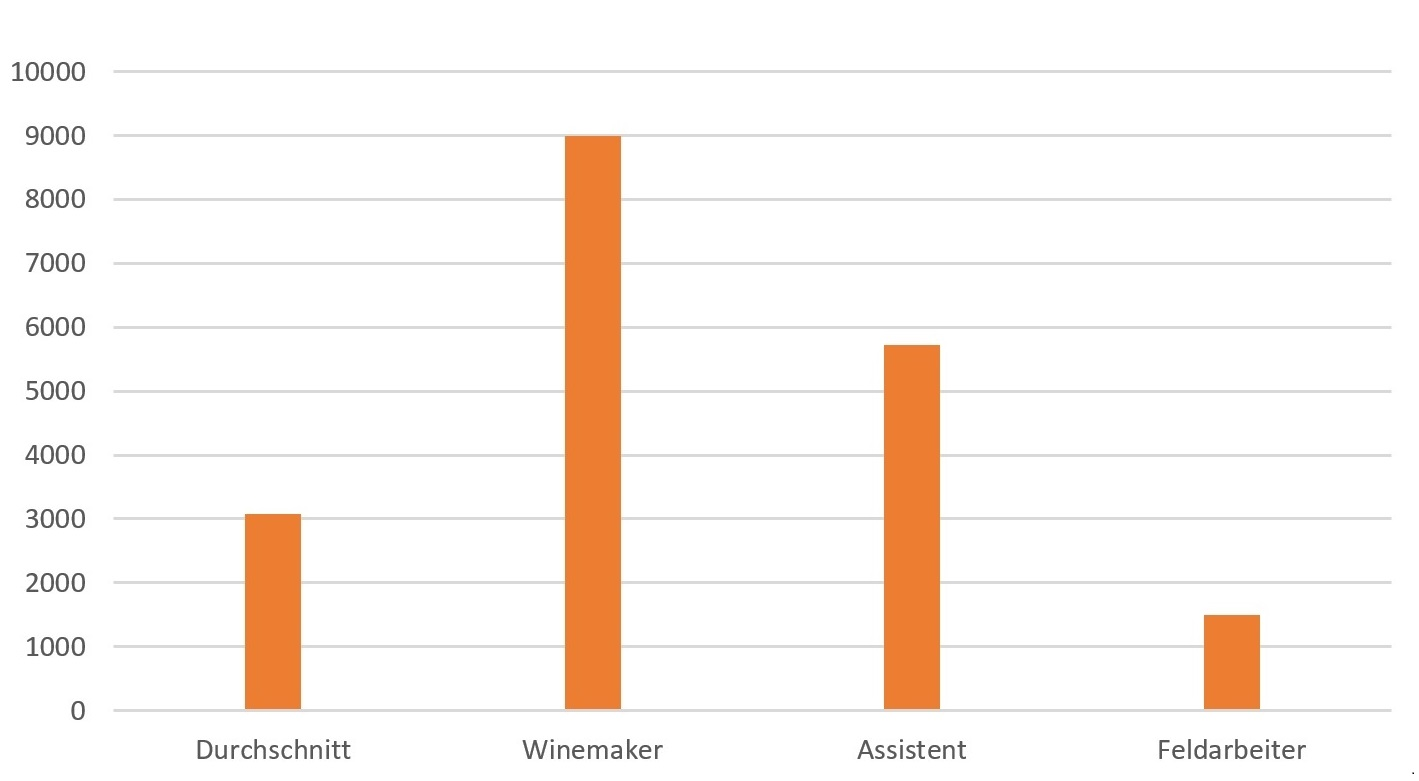
\includegraphics[width=0.9\textwidth]{Grafikarbeiter}
	\caption{Löhne der Arbeiter in der Weinproduktion}
\end{figure}
Die Arbeitsbedingungen in der USA sind im Verhältnis zur Schweiz rückständig, so hat ein Arbeitsnehmer in den USA praktisch keinen Kündigungsschutz. Dies liegt an der grossen Mobilität an den Amerikanern. Die Amerikaner haben aber Anspruch auf eine Rente, welche sie ähnlich der Schweiz mit ihrem Lohn bezahlen. \cite{_arbeitszeiten} Wie man unschwer erkennt ist das ein Feldarbeiter in Kalifornien unterbezahlt. Hier liegt auch ein grosses Verbesserungspotenzial. Ein gerechter Mindestlohn der per Gesetz geregelt ist, ähnlich wie in der Schweiz, würde die Lage für viele der Feldarbeiter stark verbessern. Zu beachten ist dass ein Feldarbeiter im Schnitt nur ein Monat auf den Feldern arbeitet, so ist eher eine Temporäre Anstellung und eine Gesetzgebung könnte sich als schwer gestalten, denn je nach Ernte und Jahr  müssen die Winzer flexibel reagieren können. In Kalifornien wird Wein seit dem 18Jh. produziert. Sowie in der Schweiz hat auch Kalifornien viele KMU Weinproduzenten. Es gibt auch einige Familienunternehmen und ebenfalls grössere Unternehmen.




	\clearpage
	\subsection{Wasser}

\subsubsection{Schweiz}
Die Schweiz wird oft als das Wasserschloss von Europa bezeichnet. «Viele wichtige Flüsse Europas – Rhein, Rhone, Inn (Donau) und Tessin (Po), Etsch (Adige) – nehmen ihren Ursprung hierzulande. Obschon die Schweiz flächenmässig nur knapp vier Promille am Kontinent ausmacht, befinden sich auf ihrem Boden sechs Prozent der Süsswasservorräte Europas». („Wasserschloss Schweiz - NZZ“, o. J.)
\begin{figure}[H]
	\centering
	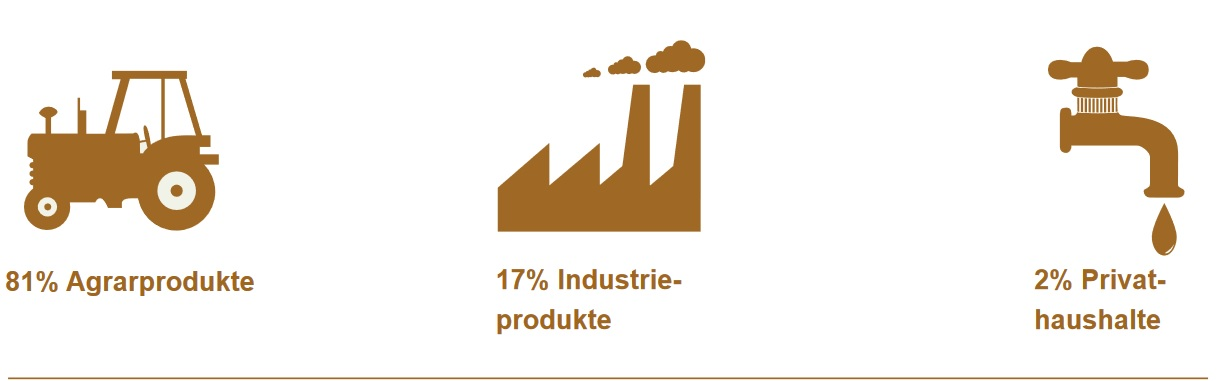
\includegraphics[width=0.9\textwidth]{WV}
	\caption{Wasserverbrauch aufgeteilt nach Sektoren}
\end{figure}
Der Gesamtwasserverbrauch in der Schweiz liegt bei 1960 Mio. $m^3/Jahr$ dieser Verbrauch teilt sich auf auf die Privathaushalte (2\%), Industrie (17\%) und auf den Agrarsektor (83\%) auf. Die Wein und Bierproduktion braucht hierzulande nur 3\% des Agrarwasserverbrauchs. Für die Weinproduktion muss in der Schweiz nur sehr wenig Wasser eingesetzt werden, da die Niederschläge meistens ausreichen. (Wettstein u. a., 2016)
\begin{figure}[H]
	\centering
	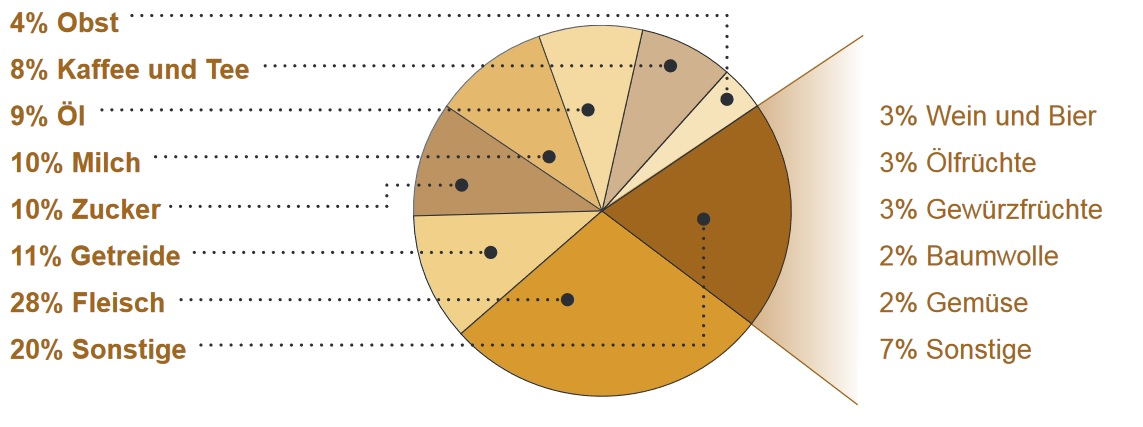
\includegraphics[width=0.9\textwidth]{WVA}
	\caption{Anteile des Wasserverbrauchs im       Agrarsektor}
\end{figure}

Durch die grosse Verfügbarkeit und die geringe Nutzung von Wasser für den Weinbau ist der Wasserverbrauch für Wein in der Schweiz nicht problematisch. Jedoch sind die Wasserverschmutzungen die durch die Weinproduktion entstehen nicht unproblematisch. Zur Wasserverschmutzung tragen vor allem Ausschwemmungen von Pestiziden bei.

\subsubsection{Kalifornien}
\label{sub:wasserverbrauch}

In Kalifornien werden etwa 42'000 $m^3$ Wasser für die Landwirtschaft benötigt. Das entspricht  39 \% des gesamten
Wasserverbrauchs. 

Der Wasserverbrauch beim Weinanbau ist grundsätzlich nicht so hoch wie bei anderen Pflanzen. Es
werden dennoch rund 700 Liter Wasser pro Liter Wein benötigt.
(\glqq{}The Water Footprint of the Wine Industry\grqq{} (2015)). 

In Kalifornien
herrscht seit 2011 eine Dürre, die Wasserrationierung nötig machte. Daher regulieren über 90 \% der
Weingüter aktiv ihre Bewässerung. Die grösste Einsparung gibt es durch die Tropfbewässerung. Dabei
wird das Wasser direkt den Wurzeln  des Weinstocks zugefügt. Dabei verdunstet weniger Wasser
unbenutzt.

Zusätzlich fliesst auch kein Wasser ab und es werden keine Nährstoffe ausgeschwemmt. Das reduziert
den Einsatz von Dünger und die Eutrophierung des Grundwassers.

Wo es der Untergrund zulässt, wird auf Trockenfeldbau gesetzt.

(\glqq{}California Wine Community Sustainability Report Appendix\grqq{} (2015)).


Auch bei der Produktion in den Kellereien wurde Massnahmen getroffen, um das verwendete Wasser zu
reduzieren. Hier fällt es vor allem für die Reinigung der Gärtanks an. Dieses Wasser wird nun
aufgefangen und wiederverwendet.

	\clearpage
	\subsection{Pestizide}
Dieser Abschnitt befasst sich um die Umweltbelastung durch Pestizide. Ein Winzer ist darauf
angewiesen die Ausfälle der Ernte möglichst klein zu halten um sein Lebensunterhalt zu finanzieren.
Ein grosser Anteil der Ausfälle ist auf Schädlinge zurückzuführen. Um Schädlinge von der Traube
fernzuhalten, wird immer wieder auf Pestizide vertraut. Dieses Verhalten bringt sofort die Frage
hervor ob durch den Einsatz von Pestiziden immer noch umweltfreundlich und nachhaltig produziert
werden. Wie in diesem Abschnitt aufgezeigt wird, gibt vor allem grosse Unterschiede ob ein Wein nach Bio oder ÖLN Standards produziert wird.
\subsubsection{Schweiz}
\begin{wrapfigure}{r}{10cm}
	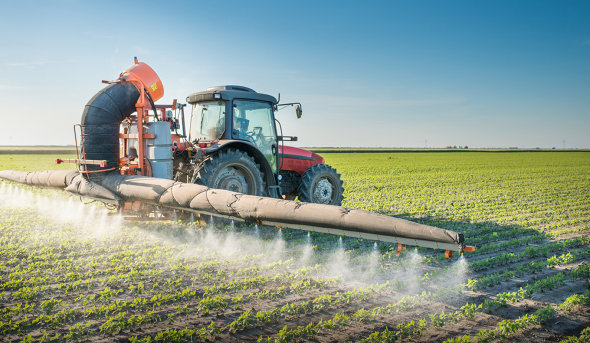
\includegraphics[width=9.5cm]{pestizide}
	\caption{Pestizide werden auf dem Feld verteilt.}
\end{wrapfigure}
In einer umfassenden Studie\\\cite{_reportweintesting-1.pdf} wurde von Greenpeace Schweiz sechs
Weinberge in verschiedenen Weinbauregionen auf Pestizide untersucht. Insgesamt wurden 33 Wirkstoffe
festgestellt von denen 23 auf der Greenpeace "Blacklist" stehen. Dies bedeutet diese Wirkstoffe sind
entweder humantoxisch oder haben eine inakzeptable Wirkung auf das Ökosystem. Zwei der gefunden
Wirkstoffe waren sogar durch die EU nicht zugelassen. In den Böden konnten ältere Pestizide
nachgewiesen werden, welches aufzeigt,  dass sich manche Pestizide nur sehr langsam abbauen und über
Jahrzehnte Schäden in den Ökosystemen anrichten. In der Studie wurden auch die fertigen Weine auf
ihre Inhalte überprüft. In der konventionellen Weinprodukten wurden vermehrt Rückstände von
Pestiziden gefunden, welche aber die Grenzwerte nicht überschritten. Allerdings gibt es für Weine auch nur selten Pestizid Grenzwerte. Wie in Abbildung \ref{fig:ha} dargestellt, ist die UBP von ÖLN ein wesentlicher Bestandteil der gesamten Belastung. Der Unterschied zur biologischen Produktion wird deutlich, die eine Anwendung von Pestiziden verbietet.
 \begin{figure}[H]	
	\centering
	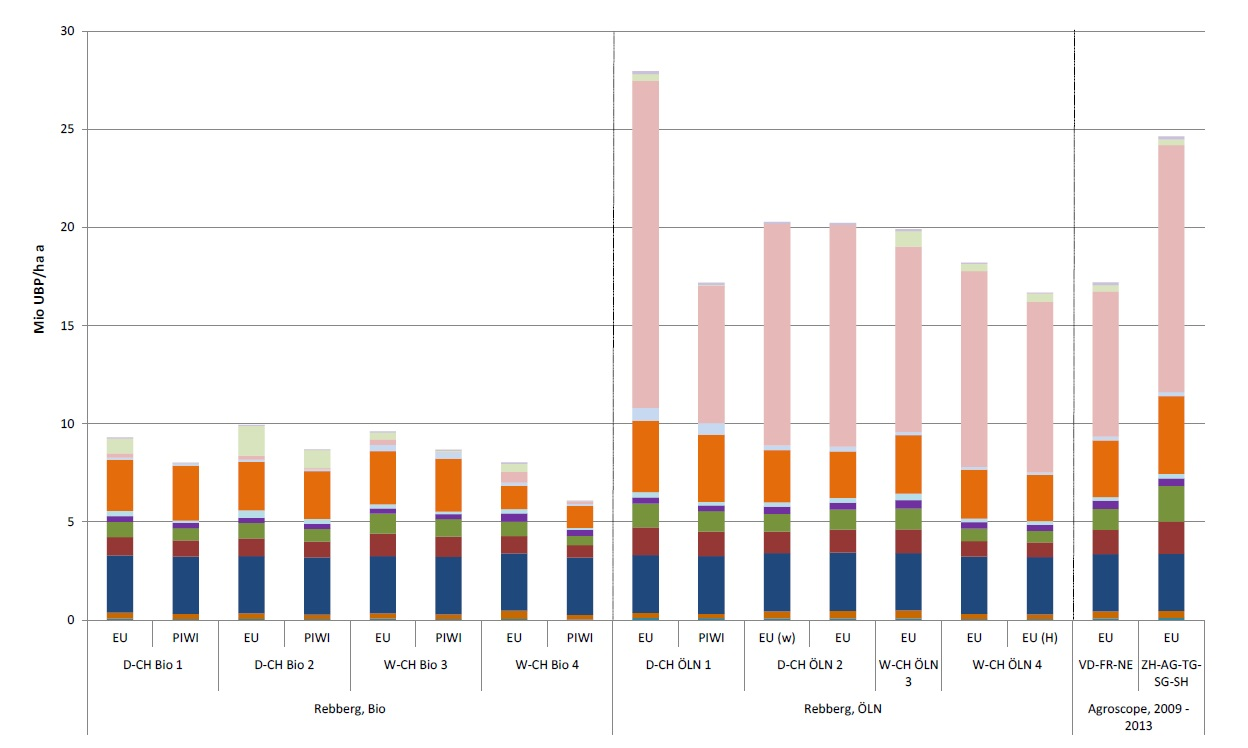
\includegraphics[width=0.9\textwidth]{auswirkungen}
	\caption{Gesamtumweltbelastung [UBP] der ÖLN- und biologischen Bewirtschaftung einer Hektare Rebbergs}
	\label{fig:ha}
\end{figure}

\subsubsection{Kalifornien}
\label{sub:sch_dlingsbek_mpfung}

Das Ziel der Schädlingsbekämpfung in Kalifornien ist nicht das komplette Ausrotten oder Verhindern
der Schädlinge. Es werden stattdessen Schwellenwerte definiert. Es werden erst Massnahmen getroffen,
wenn diese Schwellenwerte erreicht oder überschritten werden. Diese Massnahmen umfassen biologische,
kulturelle und chemische Mittel, die so eingesetzt werden, dass ökonomische, Umwelt- und
Gesundheitsrisiken minimiert werden.

Um den Einsatz von giftigen Pestiziden zu verringern, werden diese erst eingesetzt, wenn es wirklich
nötig ist. Das setzt eine kontinuierliche Kontrolle über den Schädlingsbefall voraus. Dies wird von
etwa drei Viertel der Weinbauern vorgenommen.

Als Prävention werden kulturelle Massnahmen getroffen. Dazu gehören das Entfernen von Laub, Hecken,
Staubkontrolle und Bewässerung.

\cite{_2015_cswa_sustainability_report.pdf}\\
\cite{_2015_report_appendix.pdf}


Zu den biologischen Schädlingsbekämpfungsmittel gehören natürliche Feinde wie Spinnen, Marienkäfer
oder Wespen, aber auch Hühner oder Schafe, die gegen Erdraupen oder zum Mähen von Gräsern eingesetzt
werden \cite{_sustainable}.  Durch diese Massnahmen werden weniger
Pestizide eingesetzt und die Artenvielfalt wird erhöht.

	\clearpage
	\subsection{Recycling}
Nahezu jedes Produkt welches wir kaufen hat eine Verpackung. Diese Verpackung muss ebenfalls hergestellt werden und hat somit auch eine Betrachtung bezüglich der Nachhaltigkeit nötig. In unserem Beispiel betrachten wir nur Wein welcher in Glasflaschen abgefüllt werden, welcher auch der Grossteil ausmacht welcher der Endkonsument im Laden kauft. Ausserdem werden sonstige Verpackungsmaterialen wie Karton oder Luftpolsterfolie oder Ähnliches, welche beim Transport eventuell anfallen könnten, vernachlässigt. 
Das Material Glas entsteht beim Schmelzen einer Mischung, die unter anderem Soda, Quarzsand und Kalk enthält. Das zusammenschmelzen geschieht bei etwa 1500 Grad Celsius und benötigt somit sehr viel Energie. Wird bei der Herstellung von Glas zusätzlich rezykliertes Material verwendet, so kann bis zu einem Viertel dieser Energie eingespart werden. Wichtigster Energieträger ist Erdgas bei der Produktion von Glas
\subsubsection{Schweiz}



\subsubsection{Kalifornien}
In den USA wird der meiste Abfall immer noch verbrannt oder in Deponien verscharrt. Kalifornien hat
aber eines der besten Recycling Netzwerke der Staaten. Dennoch haben nur 64\%  der Kellereien ein
Konzept zur Mülltrennung. 

Beim Recycling von Glas sieht es aber deutlich besser aus. Fast alle Kellereien trennen
wiederverwertbares Glas und fast zwei Drittel trafen Massnahmen um Glasbruch zu reduzieren.

(\glqq{}California Wine Community Sustainability Report Appendix\grqq{} (2015))

Die Recycling-Quote beim Endverbraucher hingegen ist schlecht. Sie betrug im Jahr 2015 in den ganzen
USA nur 34\%. 
	\clearpage
	\section{Vorarbeiten}
	\subsection{Analyse von den Resultaten der «Fussabdrücke»}
Der Fragebogen von WWF zeigt auf wie viele Planeten man bräuchte wenn alle Menschen denselben Lebensstill hätten, wie derjenige der diesen Fragenbogen ausfüllt. Bei unserer Gruppe lagen die Werte zwischen 2,2 und 2,9. Der Durchschnitt liegt bei 2,575. Dies bedeutet das unser durchschnittlicher Lebensstill ungefähr 2,5 Erden bräuchte.
Interessant zu sehen ist das alle der Mitglieder genau gleich viel Energie verbrauchen in den öffentlichen Diensten und dies entsprich nur ein wenig mehr als der Idealwert, bei welchen wir nur eine Erde brauchen. Bei der Mobilität, Konsum, Wohnen und Ernährung liegen alle Mitglieder unserer Gruppe im x-fachen Bereich über dem Idealwert. Bei diesen Bereichen besteht das grösste Verbesserungspotenzial. Bei der Mobilität kann man unteranderem auf einen Auslandflug verzichten. Den eine Stunde im Flugzeug entspricht circa einem Monat Autofahren. 
Ebenfalls kann man auch bei der Ernährung sich einfach verbessern. Man sollte versuchen vor allem regionale Produkte zu konsumieren. Ebenfalls ist Fleisch verzehren eine grosse Belastung für die Umwelt, dies kann jedoch simpel reduziert werden in dem man den Verzehr reduziert oder gar ganz weglässt. Was uns in der Gruppe generell erstaunt hat ist die Tatsache das Eier und Milchprodukte die Umwelt ebenfalls sehr belasten. 
Mit ein mehr Aufwand, aber ebenfalls mit grossen Potenzial, ist eine Energieeinsparung bei dem Bereich Wohnen. Eine radikale aber sehr gute Option ist es das Auswechseln einer Ölheizung zu beispielsweise einer Pelletheizung, welche einiges Umweltfreundlicher ist. Desweitern besteht auch im kleineren Aufwand Verbesserungspotenzial, beispielsweise bei den Geräten die man benutzt, sollte man darauf achten das diese in einer guten Energieklasse bewertet sind. 
Als Abschluss kann man sagen das unsere Gruppe zwar klar unter dem schweizerischen Durchschnitt liegt aber dennoch einiges machen kann um die Belastung an der Umwelt zu verringern. 

\subsection{Einkaufsverhalten}

Zur Untersuchen des Konsumverhaltens wurden vorgängig unabhängig von der Gruppe Daten erfasst zu dem Konsumverhalten der einzelnen Studenten. Genauer gesagt wurde über eine Woche untersucht, von wo die Lebensmittel genau bezogen werden. Durch das Analysieren der Daten resultiere die Grafik. Daraus ist klar ersichtlich das der Grossteil der Produkte von Grosshändler wie Migros und Coop bezogen werden.
 \begin{figure}[H]
	\centering
	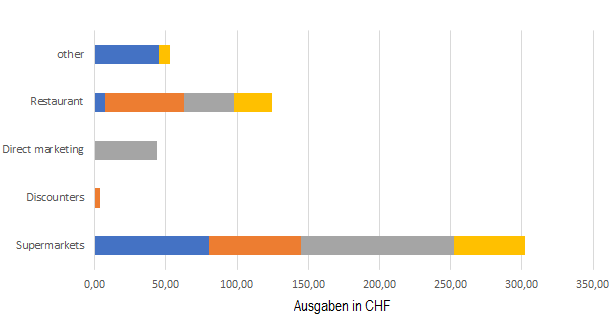
\includegraphics[width=0.9\textwidth]{ta}
	\caption{Analyse des Einkaufverhalten der einzelnen Studierenden}
\end{figure}
Diskussionen in der Gruppe hat ergab das die Hauptgründe dafür vor allem die Verfügbarkeit und die grosse Auswahl ist. Es kristallisierte sich heraus, dass die durch die Analyse der Auswahl von den verfügbaren Quellen ist, vor allem der Aspekt das Migros und Coop mittlerweile sehr viel regionale und nachhaltige Produkte im Sortiment vertreten sind ins Auge gefallen. Somit ist  das Streben nach Nachhaltigkeit nicht nach der frage, wo wir einkaufen, sondern was wir einkaufen zu klären, weil die Art der Produkte ein viel grösserer Einfluss darauf hat.
	\clearpage
	\section{Summaries}
\subsection{COOP – Strategies for Sustainable Food}

Coop is one of the largest retailers in Switzerland. Coop can look back on a History spanning over 150 years. Coop is still a cooperative because some several advantages, for example: for sustainability and long-term thinking. The Strategic concept for sustainability by Coop stand on three columns, which are:\\

-Sustainable assortment performance\\
-Resource efficiency and climate protection\\
-Employees and society\\

All these points are equally important for a company that wants to act sustainably.
In the long history of Coop, they had some milestones about sustainability. For example in 1993, Coop launched Naturaplan, Naturaline and Max Havelaar. 
The Max Havelaar foundation, which is the most famous of Coops launched foundations, is a NGO, which stand for fair-trade, and awards the fair-trade label for sustainable and fair-trade products. The benefits of this organisation is to improve the livelihood of the developing world. You can find these labels on different products such as honey, coffee, tea, bananas, cacao, cotton, pineapples, flowers, mango, orange juice, rice and sugar.
In addition, a big point in the sustainable food strategies by Coop is the thematic about the palm oil. Many areas, which are now palm oil farms, were once rainforests. So many farmers used to burn the rainforest down to increase the amount of the palm oil. Coop is very focused on selling only products from sustainable palm oil cultivation. On this point Coop is working together with the WWF to get on this goal.
For Coop Sustainable palm oil means:
– No uprooting of virgin forests and valuable living space
– Protection of water, soil, air, animals and plants
– Compliance with land use‐ and proprietary‐rights
– No child work, involving small farmers.

Coop is not only trying to sell sustainable products but also to be sustainable. For example, they want to be CO2 Neutral by the year 2023. 
In order to achieve this goal, those used, for example, to transport the goods trucks, which are driven with hydrogen instead of using conventional fuel. 

From 2003 on, they spend each year 10 Million Swiss Francs into the Foundation of Coop Naturaplan‐fund. In addition Coop spend also 16,6 Million Swiss Francs in about 70 projects which have different goals such as innovations, Raising awareness of broad public by broad communication concerning sustainability and also Compensation of CO2‐emissions.

Coop is also committed to sustainability in the social field. This is done for different reasons. One part of the unsold food will be donated to the {}\grqq Swiss table{}\grqq and {}\grqq Tischlein deck dich{}\grqq . Another aspect is that Coop also draws attention to sustainable products, and not least by labels, which have been launched by their own. As mentioned earlier in the text, Coop has launched some own labels.  For Coop, it is also a big concern to be able to infomate its customers and lables are there a good way.

Overall, Coop is a company that is very concerned about sustainability and has been around for a long time. Coop also has ambitious future plans and sustainability is also being improved in various areas.

	\clearpage
	\section{Reflexion – Blockwoche Nachhaltigkeit }
In der ersten Woche vom Februar 2017 fand die Blockwoche zum Thema Nachhaltigkeit statt. Die Blockwoche, die ebenfalls ein ISA Modul ist, wurde auf Englisch durchgeführt. Vorgängig hat jeder Teilnehmer und Teilnehmerin einen Fussabdruck von WWF erstellen lassen, bei welchen man herauslesen konnte wie nachhaltig man mit dem Planeten Erde umgeht. Des Weitern wurden Texte gelesen um einen ersten Überblick in das Thema zu kriegen. Die Woche war so gesehen in zwei Teile gegliedert. Der erste Teil waren die verschiedenen Vorlesungen von Experten und der zweite Teil war die Gruppenarbeit bei welchen wir ein Produkt genau unter die Lupe nahmen um dann am Freitag unsere Ergebnisse im Plenum zu präsentieren. Ausserdem wurde ein sogenannter «Final Report» über dieses Produkt geschrieben. Generell ging es bei dem Modul über die Nachhaltigkeit über die Nachhaltigkeit von Lebensmittel. 
Die erste «Keynote» Vorlesung war von Brigitte Zogg welche uns das Thema Nachhaltigkeit bei Coop näherbrachte. Es wurden unter anderem die Programme welche Coop unterschützt vorgestellt, wie auch die verschiedenen Labels welche auf Produkten bei Coop zu finden sind. Am Nachmittag ergänzte Jens Geissel noch zu den Labels und zeigte wie viel Information man über ein Produkt herausfinden kann innerhalb von 15 Minuten. Ebenfalls am Nachmittag zeigte Julius Gallati seine Analyse zu den «Fussabdrücken» welche wir vorgängig gemacht haben. 
Am Dienstag wurde hauptsächlich über «GMO» und «Biofuel» diskutiert. Aber es gab eine weitere Vorlesung von Albrecht Ehrensperger welche sich mit «Sustainable Development» und «Food Security» befasste. 
Am Mittwoch ging es weiter mit der «Keynote» Vorlesung von Julius Gallati welche uns vorbereitete auf die kommende Gruppenarbeit. Wie bereits erwähnt war die erste Aufgabe der Gruppe Informationen über ihr Produkt zu sammeln, in unserem Fall Wein, und diese dann zu einer Präsentation am Freitagmorgen zusammen zu tragen. Mittwochnachmittag und Donnerstag wurde hauptsächlich an dem Vortrag gearbeitet und am Freitagmorgen präsentiert. 

Die Woche gestaltete sich in zwei Teile, als Wissen vermittelt zu bekommen und Wissen zu erarbeiten.  Die ersten zwei Tage waren durch den schier endlosen Strom an Informationen sehr anspruchsvoll. Die Diskussion zwischen Pro- und Contra-Parteien bezüglich «GMO» und «BioFuel» am Dienstagnachmittag war demnach eine Auflockerung. Auch wenn wir zuerst ein wenig skeptisch waren, so lernten wir viel über die Problematik der beiden Themen. Bei der Vorlesung von Brigitte Zogg störte uns ein wenig das die Präsentation sich nie kritisch mit den Programmen von Coop auseinandergesetzt hatte. Es war zwar sehr informativ aber auch mehr Werbung für Coop als dass es wirklich kritisch betrachtet wurde. Wir hätten uns mehr gewünscht das man beispielsweise auch Labels kritisch hinterfragt hat, wie dies Jens Geisel am Nachmittag dann «nachgeholt» hat. 
Für die Gruppenarbeiten wurde genügend Zeit bereitgestellt und eine angenehme Arbeitsumgebung welche wir sehr schätzten. 

Wir denken das diese Woche ein Erfolg war, weil wir lernten das Nachhaltigkeit sehr viele Aspekte hat und deshalb fast immer eine komplexe Lösung braucht, um nicht die Probleme zu verlagern. Wir sahen viele Innovative Lösungen wie zum Beispiel, das «Laser-Leveling» welches es ermöglicht den Wasserverbrauch massiv zu verringern. Wir als Gruppe lernten natürlich viel über die Umweltaspekte von Wein.

	\clearpage
	\listoffigures
	\newpage
    \nocite{*}
    \bibliographystyle{apacite}
    \bibliography{bibliography}
\end{document}
